\iffalse
\let\negmedspace\undefined
\let\negthickspace\undefined
\documentclass[journal,12pt,onecolumn]{IEEEtran}
\usepackage{cite}
\usepackage{amsmath,amssymb,amsfonts,amsthm}
\usepackage{algorithmic}
\usepackage{graphicx}
\usepackage{textcomp}
\usepackage{xcolor}
\usepackage{multirow}
\usepackage{txfonts}
\usepackage{listings}
\usepackage{enumitem}
\usepackage{mathtools}
\usepackage{gensymb}

\usepackage{tkz-euclide} % loads  TikZ and tkz-base
\usepackage{listings}



\newtheorem{theorem}{Theorem}[section]
\newtheorem{problem}{Problem}
\newtheorem{proposition}{Proposition}[section]
\newtheorem{lemma}{Lemma}[section]
\newtheorem{corollary}[theorem]{Corollary}
\newtheorem{example}{Example}[section]
\newtheorem{definition}[problem]{Definition}
%\newtheorem{thm}{Theorem}[section] 
%\newtheorem{defn}[thm]{Definition}
%\newtheorem{algorithm}{Algorithm}[section]
%\newtheorem{cor}{Corollary}
\newcommand{\BEQA}{\begin{eqnarray}}
\newcommand{\EEQA}{\end{eqnarray}}
\newcommand{\system}[1]{\stackrel{#1}{\rightarrow}}

\newcommand{\define}{\stackrel{\triangle}{=}}
\theoremstyle{remark}
\newtheorem{rem}{Remark}
%\bibliographystyle{ieeetr}
\begin{document}
%
\providecommand{\pr}[1]{\ensuremath{\Pr\left(#1\right)}}
\providecommand{\prt}[2]{\ensuremath{p_{#1}^{\left(#2\right)} }}        % own macro for this question
\providecommand{\qfunc}[1]{\ensuremath{Q\left(#1\right)}}
\providecommand{\sbrak}[1]{\ensuremath{{}\left[#1\right]}}
\providecommand{\lsbrak}[1]{\ensuremath{{}\left[#1\right.}}
\providecommand{\rsbrak}[1]{\ensuremath{{}\left.#1\right]}}
\providecommand{\brak}[1]{\ensuremath{\left(#1\right)}}
\providecommand{\lbrak}[1]{\ensuremath{\left(#1\right.}}
\providecommand{\rbrak}[1]{\ensuremath{\left.#1\right)}}
\providecommand{\cbrak}[1]{\ensuremath{\left\{#1\right\}}}
\providecommand{\lcbrak}[1]{\ensuremath{\left\{#1\right.}}
\providecommand{\rcbrak}[1]{\ensuremath{\left.#1\right\}}}
\newcommand{\sgn}{\mathop{\mathrm{sgn}}}
\providecommand{\abs}[1]{\left\vert#1\right\vert}
\providecommand{\res}[1]{\Res\displaylimits_{#1}} 
\providecommand{\norm}[1]{\left\lVert#1\right\rVert}
%\providecommand{\norm}[1]{\lVert#1\rVert}
\providecommand{\mtx}[1]{\mathbf{#1}}
\providecommand{\mean}[1]{E\left[ #1 \right]}
\providecommand{\cond}[2]{#1\middle|#2}
\providecommand{\fourier}{\overset{\mathcal{F}}{ \rightleftharpoons}}
\newenvironment{amatrix}[1]{%
  \left(\begin{array}{@{}*{#1}{c}|c@{}}
}{%
  \end{array}\right)
}
%\providecommand{\hilbert}{\overset{\mathcal{H}}{ \rightleftharpoons}}
%\providecommand{\system}{\overset{\mathcal{H}}{ \longleftrightarrow}}
	%\newcommand{\solution}[2]{\textbf{Solution:}{#1}}
\newcommand{\solution}{\noindent \textbf{Solution: }}
\newcommand{\cosec}{\,\text{cosec}\,}
\providecommand{\dec}[2]{\ensuremath{\overset{#1}{\underset{#2}{\gtrless}}}}
\newcommand{\myvec}[1]{\ensuremath{\begin{pmatrix}#1\end{pmatrix}}}
\newcommand{\mydet}[1]{\ensuremath{\begin{vmatrix}#1\end{vmatrix}}}
\newcommand{\myaugvec}[2]{\ensuremath{\begin{amatrix}{#1}#2\end{amatrix}}}
\providecommand{\rank}{\text{rank}}
\providecommand{\pr}[1]{\ensuremath{\Pr\left(#1\right)}}
\providecommand{\qfunc}[1]{\ensuremath{Q\left(#1\right)}}
	\newcommand*{\permcomb}[4][0mu]{{{}^{#3}\mkern#1#2_{#4}}}
\newcommand*{\perm}[1][-3mu]{\permcomb[#1]{P}}
\newcommand*{\comb}[1][-1mu]{\permcomb[#1]{C}}
\providecommand{\qfunc}[1]{\ensuremath{Q\left(#1\right)}}
\providecommand{\gauss}[2]{\mathcal{N}\ensuremath{\left(#1,#2\right)}}
\providecommand{\diff}[2]{\ensuremath{\frac{d{#1}}{d{#2}}}}
\providecommand{\myceil}[1]{\left \lceil #1 \right \rceil }
\newcommand\figref{Fig.~\ref}
\newcommand\tabref{Table~\ref}
\newcommand{\sinc}{\,\text{sinc}\,}
\newcommand{\rect}{\,\text{rect}\,}
%%
%	%\newcommand{\solution}[2]{\textbf{Solution:}{#1}}
%\newcommand{\solution}{\noindent \textbf{Solution: }}
%\newcommand{\cosec}{\,\text{cosec}\,}
%\numberwithin{equation}{section}
%\numberwithin{equation}{subsection}
%\numberwithin{problem}{section}
%\numberwithin{definition}{section}
%\makeatletter
%\@addtoreset{figure}{problem}
%\makeatother

%\let\StandardTheFigure\thefigure
\let\vec\mathbf

\bibliographystyle{IEEEtran}





\bigskip



\title{GATE ECE 2023}
\author{Karyampudi Meghana Sai\\ EE23BTECH11031}
\maketitle
Consider a discrete-time signal with period $N=5$. Let the discrete-time Fourier series (DTFS) representation be $x[n]=\sum\limits_{k=0}^{4} a_k e^{\frac{jk2\pi n}{5}}$, where $a_0=1$, $a_1=3j$, $a_2=2j$, $a_3=-2j$, $a_4=-3j$. The value of the sum $\sum\limits_{n=0}^{4}x[n] \sin\brak{\frac{4\pi n}{5}}$ is\\
(A) -10\\
(B) 10\\
(C) -2\\
(D) 2\\
\hfill Gate 2023 EC 47

\solution\\
\fi
\begin{enumerate}
\item Solving the question for N=5:
\begin{table}[h!]
 	\centering
 	\resizebox{6 cm}{!}{
 		\begin{tabular}{|c|c|c|}
    \hline
    \textbf{Parameter} & \textbf{Value} & \textbf{Description} \\[6pt]
    \hline
    $N$ &  $5$ & Time period \\ \cline{1-2}\cline{3-3}
    $X(k)$ & $\sum\limits_{n=0}^{N-1} x(n)e^{\frac{-j2\pi kn}{N}}$ & DFT formula\\ \cline{1-2}\cline{3-3}
    $X(0)$ &  $5$ & \multirow{5}{*}{\begin{tabular}[c]{@{}c@{}}DFT\\ values\end{tabular}} \\ \cline{1-2}
    $X(1)$ &  $15j$ &    \\ \cline{1-2}
    $X(2)$ &  $10j$ &    \\ \cline{1-2}
    $X(3)$ &  $-10j$ &    \\ \cline{1-2}
    $X(4)$ &  $-15j$ &    \\ \hline 
\end{tabular}

 	}
 	\vspace{6 pt}
 	\caption{Input Parameters}
 	\label{tab:gate23ec47tab2}
 \end{table} 
\begin{align}
\sum\limits_{n=0}^{4}x(n) \sin\brak{\frac{4\pi n}{5}}&=\sum\limits_{n=0}^{4}x(n)\sbrak{\frac{e^{\frac{j4\pi n}{5}}-e^{\frac{-j4\pi n}{5}}}{2j}}\\
&=\frac{1}{2j}\sbrak{\sum\limits_{n=0}^{4}x(n)e^{\frac{j2\pi (2)n}{5}}-\sum\limits_{n=0}^{4}x(n)e^{\frac{-j2\pi (2)n}{5}}}\label{eq:gate23ec47eq2}
\end{align}

Refering to the table \ref{tab:gate23ec47tab2}.\\
\begin{align}
X(k)&=\sum\limits_{n=0}^{4} x(n)e^{\frac{-j2\pi kn}{5}}\label{eq:gate23ec47eq3}
\end{align}
Referencing from equation \eqref{eq:gate23ec47eq3}, equation \eqref{eq:gate23ec47eq2} can be written as:
\begin{align}
\sum\limits_{n=0}^{4}x(n) \sin\brak{\frac{4\pi n}{5}}&=\frac{1}{2j}\sbrak{X(-2)-X(2)}\label{eq:gate23ec47eq4}
\end{align}
From the property of discrete Fourier series.\\
\begin{align}
X(k)=X(k+N)
\end{align}
So, equation \eqref{eq:gate23ec47eq4} becomes,\\
\begin{align}
\sum\limits_{n=0}^{4}x(n) \sin\brak{\frac{4\pi n}{5}}&=\frac{1}{2j}\sbrak{X(3)-X(2)}\\
\sum\limits_{n=0}^{4}x(n) \sin\brak{\frac{4\pi n}{5}}&=-10
\end{align}
\begin{figure}[htbp]
    \centering
    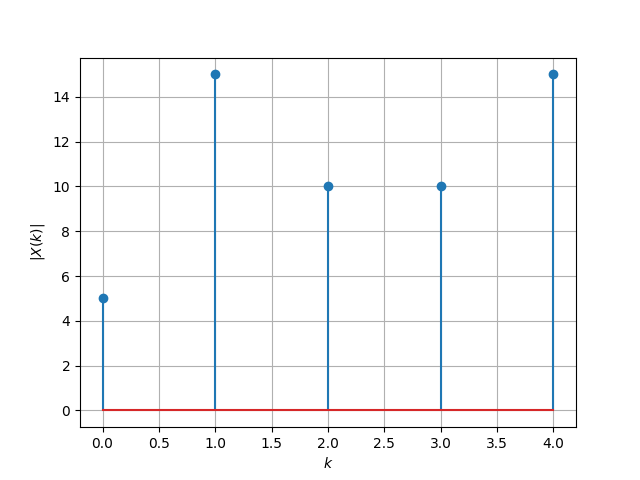
\includegraphics[width=\columnwidth]{2023/EC/47/figs/mm1.png}
    \caption{Amplitude of equation \eqref{eq:gate23ec47eq3}}
    \label{fig:gate23ec47fig1}
\end{figure}
\begin{figure}[htbp]
    \centering
    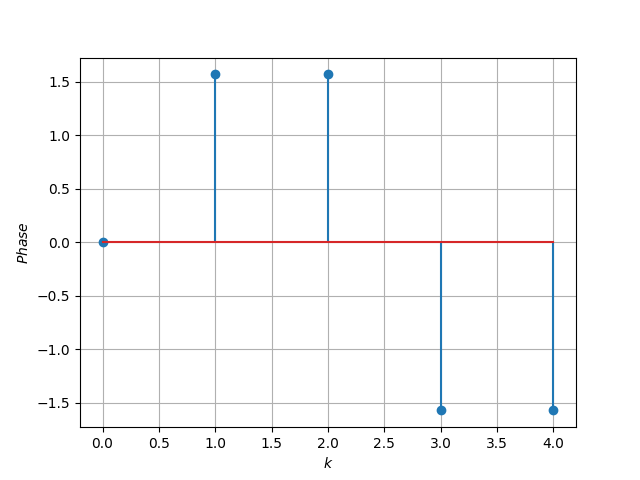
\includegraphics[width=\columnwidth]{2023/EC/47/figs/mm11.png}
    \caption{Phase of equation \eqref{eq:gate23ec47eq3}}
    \label{fig:gate23ec47fig2}
\end{figure}

\item Solving the question for N=8:
\begin{table}[h!]
 	\centering
 	\resizebox{6 cm}{!}{
 		\begin{tabular}{|c|c|c|}
    \hline
    \textbf{Parameter} & \textbf{Value} & \textbf{Description} \\[6pt]
    \hline
    $N$ &  $8$ & Time period \\ \cline{1-2}\cline{3-3}
    $X(k)$ &  $\sum\limits_{n=0}^{N-1} x(n)e^{\frac{-j2\pi kn}{N}}$ & DFT formula\\ \cline{1-2}\cline{3-3}
    $X(0)$ &  $8$ & \multirow{5}{*}{\begin{tabular}[c]{@{}c@{}}DFT \\ values\end{tabular}} \\ \cline{1-2}
    $X(1)$ &  $24j$ &    \\ \cline{1-2}
    $X(2)$ &  $16j$ &    \\ \cline{1-2}
    $X(3)$ &  $-16j$ &    \\ \cline{1-2}
    $X(4)$ &  $-24j$ &    \\ \cline{1-2}
    $X(5)$ &  $0$ &    \\ \cline{1-2}
    $X(6)$ &  $0$ &    \\ \cline{1-2}
    $X(7)$ &  $0$ &    \\ \hline
\end{tabular}

 	}
 	\vspace{6 pt}
 	\caption{Input Parameters}
 	\label{tab:gate23ec47tab1}
 \end{table} 
\begin{align}
\sum\limits_{n=0}^{7}x(n) \sin\brak{\frac{4\pi n}{8}}&=\sum\limits_{n=0}^{7}x(n)\sbrak{\frac{e^{\frac{j4\pi n}{8}}-e^{\frac{-j4\pi n}{8}}}{2j}}\\
&=\frac{1}{2j}\sbrak{\sum\limits_{n=0}^{7}x(n)e^{\frac{j2\pi (2)n}{8}}-\sum\limits_{n=0}^{7}x(n)e^{\frac{-j2\pi (2)n}{8}}}\label{eq:gate23ec47eq9}
\end{align}

Refering to the table \ref{tab:gate23ec47tab1}.
\begin{align}
X(k)&=\sum\limits_{n=0}^{7} x(n)e^{\frac{-j2\pi kn}{8}}\label{eq:gate23ec47eq10}
\end{align}
Referencing from equation\eqref{eq:gate23ec47eq10}, equation\eqref{eq:gate23ec47eq9} can be written as:
\begin{align}
\sum\limits_{n=0}^{7}x(n) \sin\brak{\frac{4\pi n}{8}}&=\frac{1}{2j}\sbrak{X(-2)-X(2)}\label{eq:gate23ec47eq11}
\end{align}
From the property of discrete Fourier series.\\
\begin{align}
X(k)=X(k+N)
\end{align}
So, equation\eqref{eq:gate23ec47eq11} becomes,\\
\begin{align}
\sum\limits_{n=0}^{7}x(n) \sin\brak{\frac{4\pi n}{8}}&=\frac{1}{2j}\sbrak{X(6)-X(2)}\\
\sum\limits_{n=0}^{7}x(n) \sin\brak{\frac{4\pi n}{8}}&=-8
\end{align}
\begin{figure}[h!]
    \centering
    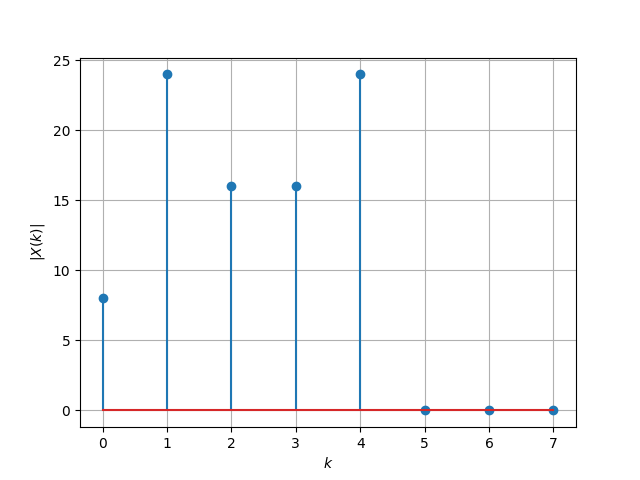
\includegraphics[width=\columnwidth]{2023/EC/47/figs/mm2.png}
    \caption{Amplitude of equation \eqref{eq:gate23ec47eq10}}
    \label{fig:gate23ec47fig3}
\end{figure}
\begin{figure}[h!]
    \centering
    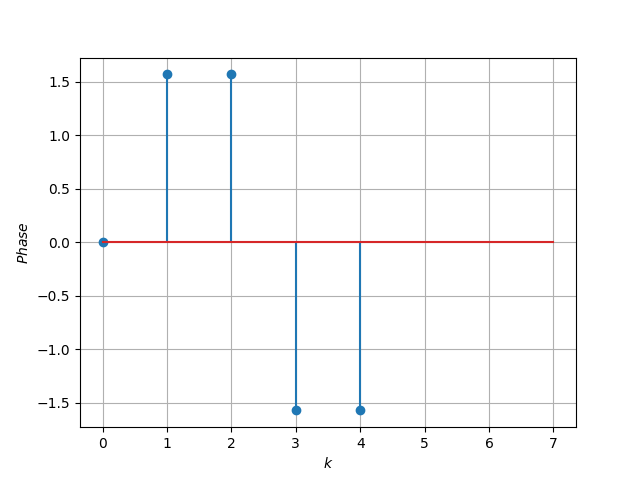
\includegraphics[width=\columnwidth]{2023/EC/47/figs/mm21.png}
    \caption{Phase of equation \eqref{eq:gate23ec47eq10}}
    \label{fig:gate23ec47fig4}
\end{figure}

\end{enumerate}

%\end{document}
